\documentclass{beamer}
\usepackage[version=4]{mhchem} 



\usetheme{Madrid}
\usecolortheme{beaver}

\title{Unit 3}
\subtitle{Modeling Atomic Structure}
\author{Mr. Maxwell}
\institute{PACS}
\date{\today}


\begin{document}

\frame{\titlepage}

\section{Atomic Structure}

\begin{frame}

    \frametitle{Número atómico}
    \onslide El 
     \pause \alert{número atómico}
     \onslide es el número de 
     \pause \alert{protones} 
     Deslizamiento en el núcleo de un átomo.
\end{frame}


\begin{frame}

    \frametitle{Masa atómica}
    \onslide El 
     \pause \alert{número masivo}
     \onslide el número total de
     \pause \alert{protones} 
     \onslide y
     \pause \alert{neutrones} 
     Deslizamiento en el núcleo de un átomo.

    \end{frame}

\begin{frame}

    \frametitle{Hidrógeno}
    $$\ce{^{\alert{1}}_{}H}$$

    \pause ¿Qué significa \alert{1}?
    \pause 1 es el número total de neutrones y protones.
\end{frame}


\begin{frame}

    \frametitle{Helio}
 $$\ce{^{4}_{2}He}$$

 \pause ¿Qué significa \alert{4}?
 \pause \alert{4} es el número total de neutrones y protones.
 \pause ¿Qué significa \alert{2}?
 \pause \alert{2} es el número de protones.

\end{frame}

\begin{frame}

    \frametitle{Litio}
 $$\ce{^{7}_{3}Li}$$

 \pause ¿Cuántos protones tiene el litio?
 \pause 3
 \pause ¿Cuántos neutrones?
 \pause $7 - 3 = \pause 4 $
\end{frame}

\subsection{Bohr Model}

\begin{frame}
    \begin{columns}
        \frametitle{The Great Dane}
        \begin{column}{0.5\textwidth}
            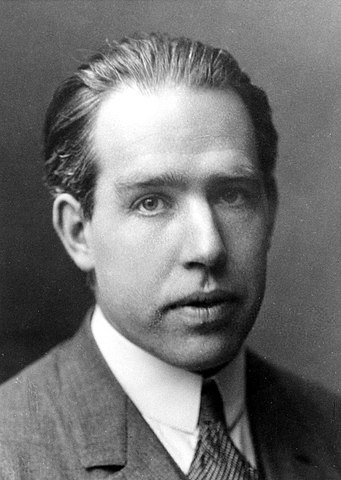
\includegraphics[width=3cm]{../../../../public/images/Bohr.jpg}
        \end{column}
        \begin{column}{0.5\textwidth}
            El modelo de Bohr: Bohr propuso que un átomo era un núcleo con electrones "orbitando" en diferentes 
            \pause \alert{niveles de energía}.
            \vspace{1cm}
        
        \end{column}
    \end{columns}
\end{frame}

\begin{frame}
    
    \frametitle{Energy Levels}
    \onslide The electrons closest to the nucleus have the 
    \pause \alert{lowest} 
    \onslide energy, while those further from away have 
    \pause\alert{higher} 
    \onslide energy.
\end{frame}

\begin{frame}
    \frametitle{Nitrogen}
    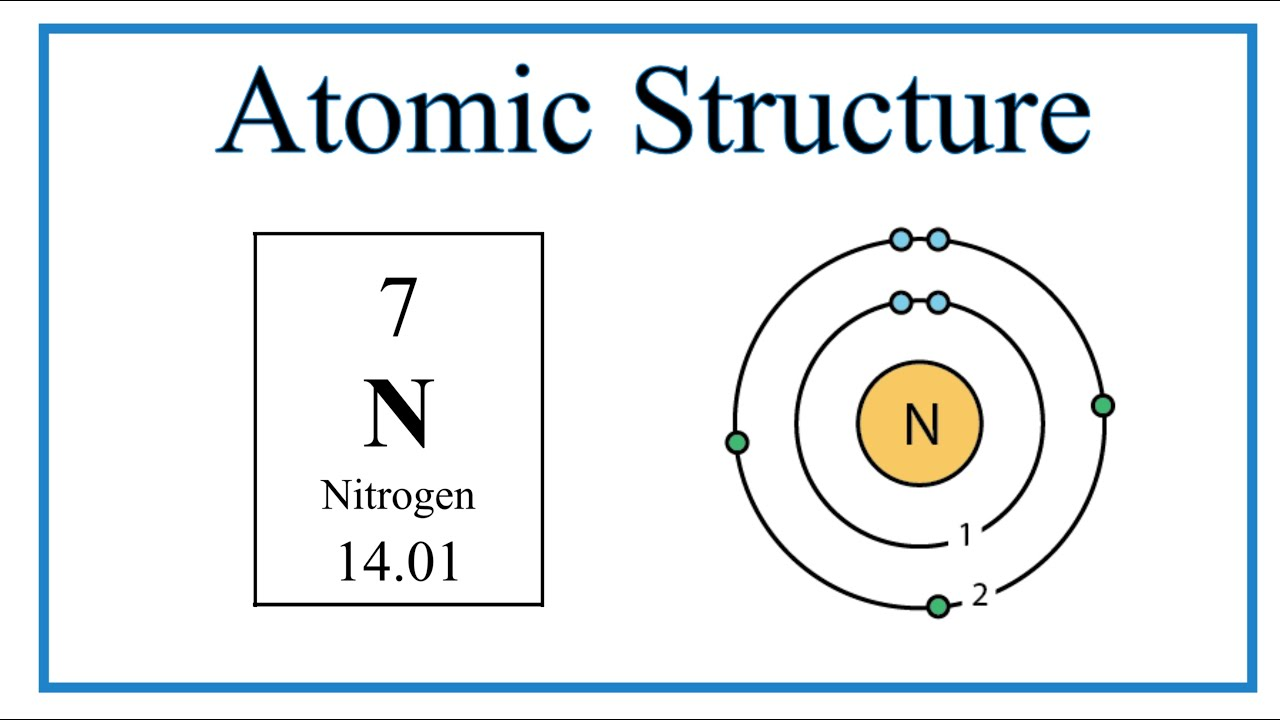
\includegraphics[width=4cm]{../../../../public/images/bohr_atom_N.jpg}
\end{frame}


\end{document}